\subsection{Dipoles}
Modeling the electromagnetic radiation from antennas is a challenging task. Employing magnetic and electric dipoles is an effective approach, particularly for electrically small antennas. They are defined as antennas with dimensions much less than one-tenth of the wavelength ($<<\frac{\lambda}{10}$)\cite{Balanis_1997}. By calculating the respective dipole moments, the coupling between antennas and TEM cells can be numerically estimated. This section provides a brief introduction to the underlying theory of this concept.

\subsubsection{Electric Dipoles}
An electric dipole is often described as two tiny charged metal spheres, which are connected with a linear and thin wire \cite{Griffiths_2024} or simply as an T-antenna containing charged capacitor-plates at the ends of the wire \cite{Balanis_1997}. The distance $d$ between those charges is very short compared to the wavelength ($d << \lambda$).%, therefore the dipole can be approximated as ideal\cite{Griffiths_2024}. 
The electric dipole moment $\mathbf{p}$ is defined by the product of charges and their separation distance, as expressed in \autoref{eqn:elec_dipole_mom}\cite{Balanis_1997,Jackson}. %% Erklärung hier. Besser die Bücher zu referenzieren, als selbst etwas zu erfinden.

\begin{equation}
    \mathbf{p} = \iiint\mathbf{x'} \rho (\mathbf{x'})\mathrm{d}^3x'
    \label{eqn:elec_dipole_mom}
\end{equation}

\autoref{fig:electric_dipole} demonstrates a simple center-fed wire antenna with a narrow gap as the feedpoint. Since the wire is electrically small and very thin, it can be accurately modeled as an electric dipole \cite{Griffiths_2024,Jackson}. A current $I_0$ is injected at the feedpoint, which linearly drops to zero along the antenna arms, as described by \autoref{eqn:current_dipole}\cite{Jackson}.

\begin{equation}
    I(z)= I_0\left( 1-\frac{2|z|}{d} \right)
    \label{eqn:current_dipole}
\end{equation}

%Hier das Ergebnis der Integration anschreiben. Die integration selbst auch anschreiben- 

\begin{figure}[h]
    \centering
    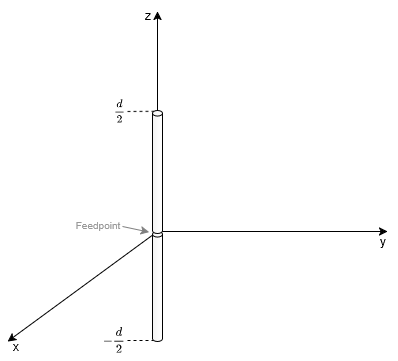
\includegraphics[width=0.5\linewidth]{Documentation//images/electric_dipole_drawing.png}
    \caption{Electric dipole}
    \label{fig:electric_dipole}
\end{figure}

Charge accumulates along the antenna's arms and is expressed as a charge per unit length $\rho'$. The charge distribution $\rho'$ is derived by the continuity equation in frequency domain, as shown in \autoref{eqn:charge_distribution_dipole}. It is uniformly distributed along each antenna arm \cite{Griffiths_2024,Jackson}.

\begin{equation}
    \rho' = \pm\frac{\mathrm{d}}{\mathrm{d}z}\frac{\mathrm{i}I(z)}{\omega} = \pm\frac{2\mathrm{i}I_0}{\omega d}
    \label{eqn:charge_distribution_dipole}
\end{equation}

Knowing the charge distribution $\rho'$ enables the calculation of the electric dipole moment $\mathbf{p}$ using \autoref{eqn:elec_dipole_mom}. This results in \autoref{eqn:dipole_mom_example}. The electric dipole moment $\mathbf{p}$ is parallel to the antenna's arms and points in the z-direction \cite{Griffiths_2024}\cite{Jackson}. 

\begin{equation}
    \mathbf{p}=\int_{-\frac{d}{2}}^{\frac{d}{2}}z\rho'(z)\mathrm{d}z\cdot\mathbf{e}_z = \frac{\mathrm{i}I_0d}{2\omega}
    \label{eqn:dipole_mom_example}
\end{equation}

Next, the vector potential $\mathbf{A}$ is determined. It is generally defined in \autoref{eqn:vector_pot}\cite{Balanis_1997}\cite{Jackson}. % Eventuell extra in einem anderen Kapitel diese Bascis anschreiben. 

\begin{equation}
    \mathbf{A}(\mathbf{x})=\frac{\mu}{4\pi}\frac{\mathrm{e}^{\mathrm{i}kr}}{r}\iiint \mathbf{J}(\mathbf{x'})\mathrm{d}^3x'
    \label{eqn:vector_pot}
\end{equation}

In the case of an electric dipole, the calculations of the vector potential $\mathbf{A}$ simplifies to \autoref{eqn:vector_pot_elec_dipole}\cite{Jackson}.

\begin{equation}
    \mathbf{A} (\mathbf{x})=-\frac{\mathrm{i\mu_0\omega}}{4\pi}\mathbf{p}\frac{\mathrm{e}^{\mathrm{i}kr}}{r}
    \label{eqn:vector_pot_elec_dipole}
\end{equation}
%Should the calculation of fields even be included? I don't need them for research. But the Field equations are important for explaining the frequency behavior of the electric dipole moment. This can be done by the radiation resistance in \autoref{eqn:elec_rad_res}. In our example, the radiation power depends on the frequency squared ($\mathbf{p}$\textasciitilde

Any other field quantities can be derived out of the vector potential $\mathbf{A}$, such as the electric field strength $\mathbf{E}$ and magnetic field strength $\mathbf{H}$. \autoref{eqn:elec_and_mag_field_dipole} expresses their relation \cite{Balanis_1997}. 

\begin{subequation}\label{eqn:elec_and_mag_field_dipole}
    \begin{equation}
    \mathbf{H} = \hat{a}_{\phi} \frac{1}{\mu r} \left[ \frac{\partial}{\partial r} (r A_{\theta}) - \frac{\partial A_{r}}{\partial \theta} \right]
    \end{equation}
    
    \begin{equation}
    \mathbf{E}=-\mathrm{i}\omega\mathbf{A}-\mathrm{i}\frac{1}{\omega\mu\epsilon}\nabla\left(\nabla\cdot\mathbf{A}\right)
    \end{equation}
    
\end{subequation}

The power radiated by an antenna is determined from the time-averaged Poynting vector $ \langle \mathbf{S} \rangle$. \autoref{eqn:time_averaged_poynting} defines this quantity, where only the real part is relevant, since it represents the actual radiated power \cite{Balanis_1997}.

\begin{equation}
    \langle \mathbf{S} \rangle = \frac{1}{2} \, \Re \{ \mathbf{E} \times \mathbf{H}^* \}
    \label{eqn:time_averaged_poynting}
\end{equation}

By integrating the time-averaged Poynting vector $ \langle \mathbf{S} \rangle$ over a closed surface, the radiated power $P_{\mathrm{rad}}$ is determined. The real part of the power is independent of the integrated surface, and in case of an electric dipole is expressed as \autoref{eqn:elec_rad_res}. The radiated power increases with the frequency squared, as the antenna becomes more efficient. This relation holds, as long as the antenna is electrically small.

\begin{equation}
    P_{\mathrm{rad}} = \frac{\mathrm{c}^2\mathrm{Z_0}\mathrm{k}^4}{12\pi}|\mathbf{p}|^2
    \label{eqn:elec_rad_res}
\end{equation}

The electric dipole described in this section approximate the real behavior of electrically short antennas. However, special care must be taken of the excitation method and shape, as it influences the results heavily \cite{Jackson}. Additionally, any antenna investigated through this method must remain as small as possible compared to the wavelength $\lambda$, to reduce any analytical approximation errors. 

The electric field increases quadratically with frequency.... Hence electric dipole moment increases over frequency... Write about that -> Griffiths

\todo{Balanis image theory of dipoles}

% Next, the electric and magnetic fields, how the dipole moment is calculated with this and how ansys HFSS uses this. Look also in the other two ressources, the other two books. Ansys HFSS handles them as physical dipole antennas? Maybe add radiation pattern. Additionally, describe how the electric field odminates in electric dipoles. In Dominik's paper, the magnetic coupling dominates, because of the magnetic dipole.

% The behavior of the electric dipole may be divided into three categories\cite{Griffiths_2024,Jackson}:
% \begin{enumerate}
%     \item The near zone, 
% \end{enumerate}

\subsubsection{Magnetic Dipoles}

The magnetic dipole is modeled as a current loop with radius $b$, whose axis is perpendicular to the plane of the loop. Its radiated fields are analogous to those of an electric dipole, with the electric and magnetic fields interchanged \cite{Balanis_1997}. \autoref{fig:magnetic_dipole_drawing} shows a magnetic dipole.

\begin{figure}[h]
    \centering
    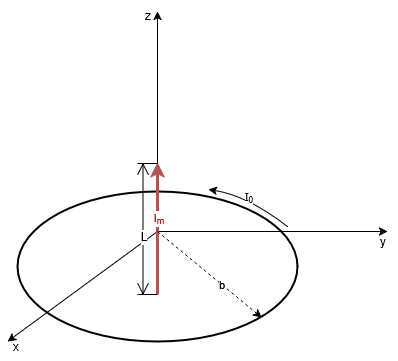
\includegraphics[width=0.5\linewidth]{Documentation//content//10_theory//img/magnetic_dipole_drawing.png}
    \caption{Magnetic dipole}
    \label{fig:magnetic_dipole_drawing}
\end{figure}

The magnetic dipole moment is given by \autoref{eqn:mag_dipole_moment}.

\begin{equation}
    \mathbf{m}=\frac{1}{2}\int (\mathbf{x} \times \mathbf{J})\mathrm{d}^3x
    \label{eqn:mag_dipole_moment}
\end{equation}

A magnetic dipole can be represented with a current loop, or a magnetic current along a straight path. \autoref{eqn:magn_current_curr_loop} shows the mathematical relation between these two \cite{Balanis_1997}. 

\begin{equation}
    I_m L = \mathrm{i}S\omega\mu_0 I_0
    \label{eqn:magn_current_curr_loop}
\end{equation}

$I_m$ is the magnetic current with the unit $\mathrm{V}$. The area $S$ of the loop is calculated by $b^2\pi$. $I_0$ is the electric current with the unit $\mathrm{A}$ flowing through the loop, and $\mu_0$ is the permeability of free space.

\todo{Add fields and radiation power formulas, if it is needed later}

\subsubsection{Crossed Dipoles}
% Read Bauernfeind's: Crossed Dipole Antennas

% When placing the magnetic dipole in the center of the upper or lower chamber of the TEM cell, and pointing in y-direction, it will generate a TEM-wave. Same goes for the electric dipole, pointing in z-direction. When combining two of these dipole moments, any excitation with the first order TEM mode is possible. This is the main idea for modeling antennas. The relation of the magnetic and electric fields is assumed to be roughly equal to the free space wave impedance. Also, magnetic dipoles create a difference in output voltage of the two ports, while electric dipoles create a increase of voltage in both ports. The power transmitted is the same. However: How are they modeled in HFSS? 

Crossed dipoles can generate a wide variety of radiation patterns. Supposed two dipoles are placed perpendicular to each other and fed 90° out of phase, an omnidirectional radiation pattern in created \cite{7293591}. If the equivalent dipoles of an EUT represents such two dipoles, any mode which can propagate in the TEM cell will do so, and therefore influence the measurement result. It is therefore not only important to know which dipoles there are representing the EUT, but also what phase and magnitude they have. Meaning that not only the dipoles aligned with the TEM mode alone influence the result. 
\todo{Write}

\todo{Dipoles next to conducting planes (balanis, collin)}

% Also, the reflections of the conducting sheets of the TEM cell might enhance the dipoles' gain, therefore artificially supporting a certain mode even more. This property is often used in antennas, where a perfect electric conductor (PEC) is placed a quarter wavelength away from the antenna, hence enhancing the gain \cite{7293591}. 

